%\documentclass[11pt, oneside]{article}										% use "amsart" instead of "article" for AMSLaTeX format
%\usepackage{geometry}													    % See geometry.pdf to learn the layout options. There are lots.
%\geometry{a4paper}													        % ... or a4paper or a5paper or ... 
%\geometry{landscape}													    % Activate for rotated page geometry
%\usepackage[parfill]{parskip}												% Activate to begin paragraphs with an empty line rather than an indent
%\usepackage{graphicx}                                                      % Use pdf, png, jpg, or eps� with pdflatex; use eps in DVI mode		
%\usepackage{amssymb}
%SetFonts
%SetFonts
%\date{}																    % Activate to display a given date or no date
%--------------------------------------------------------------------------------------------------------------------------------------------

\documentclass[journal]{IEEEtran}										    % use "amsart" instead of "article" for AMSLaTeX format
\usepackage[showframe=false]{geometry}										% See geometry.pdf to learn the layout options. There are lots.
\geometry{left=1.7cm,right=1.7cm,top=1.9cm,bottom=2cm}                      % Set margin of the paper
\usepackage[pdftex]{graphicx}													    % Use pdf, png, jpg, or eps� with pdflatex; use eps in DVI mode
\graphicspath{{img/}}
% \usepackage{blindtext}                                                      % Dummy Text
\usepackage{hyperref}                                                       % Link to Reference 

\title{\textbf{Animal Racing Video Game Using Hand Motion}}
\author{Thanut Sajjakulnukit, Nutcharueta Sihirunwong, Budnampetch Onmee \\
    \Large Kasetsart University }

\begin{document}
    % \markboth{Journal of \LaTeX\ Class Files,~Vol.~1, No.~8, April~2018}
    % {Shell \MakeLowercase{\textit{et al.}}: Bare Demo of IEEEtran.cls for IEEE Journals}
    \maketitle
    
    \begin{abstract}                                                        % Start Abstract here
        Nowadays, video games are among the best sources of entertainment 
        that people use to enjoy themselves together. In addition to the 
        entertainment, the player will also gain knowledge or skills 
        depending on the purpose of the game?s creators. We  develop a new 
        kind of game that uses Leap Motion to detect your own hands and 
        control the character movements via different gestures. 
        The Leap Motion will make game more fun, challenge, and interesting. 
        This project is not only for entertainment, but also for the 
        illustrations of animal mechanisms so that kids can learn. 
        This project also lets people participate in some activities together.

    \end{abstract}

    \section{Introduction}                                                  % Start Introduction here
        \IEEEPARstart{C}{urrently}, the social condition makes a pressure 
        on people?s stress. Video games are one of the answers to help relieve 
        stress. Today there are many developers who created the video 
        game in the market but it doesn't have a new technology to make 
        a different video game. Leap Motion is one of technology that 
        can be used with the game. It is hand tracking technology is 
        designed to be embedded directly into VR/AR headset. 

        In this project, we will use Leap Motion technology, one of
        the new technology that use virtual hand to control object
        in video game. To create a racing video game by tracking 
        hand to control character?s movement depending on the 
        physical characteristic of each animal. The movement of 
        character in the game is related to movement of the hand 
        which makes the game more challenge and interesting.
        
    \section{Literature Summary}                                            % Start literature summary here
        The research paper and publish experiment are related to video game 
        technology and creating process which is the technology that we 
        focussing on this project. The good video game should have a technique 
        associated with the story in the video game. So, the interesting 
        video game should make difficult fun in the video game to make a player 
        enjoy and make difficult with other video game \cite{TAG5} using a good engine 
        like a Unity and 3D modeling software tools to make a video game.

        The 3D modeling software has a lot; however, the popular tools is a 
        Blender and Maya \cite{TAG4}. In the research is a comparison between Maya 
        and Blender, its focus on comparing the process of two software tools 
        to make a group decision to choose blender for creating a model on 
        the game because it is user-friendly like unity3D so we might not 
        have to research from the beginner.

        And the last thing can make the game interesting is a new technology 
        that matches with our video game project. It is Leap Motion technology, 
        it can working on the variability of the sensor \cite{TAG1} to detect hand motion 
        and identify hand gesture, an Anthropomorphic Hand with five fingers 
        controlled by a Motion Leap device \cite{TAG2} and evaluate of natural user 
        interface usability based on the Leap Motion device \cite{TAG3}. All of this 
        research focuses on the stability of the different measurements which 
        can be produced either by the user or the sensor to be natural because 
        it is necessary that the user has the feeling of always being in control, 
        with minimal time and effort as possible.


        \section{Related Theory}
        In this section, we introduce the important API, design principle and algorithm
        that related to our project.

            \subsection{Leap Motion API}
                The Leap Motion is a new technology for a system recognizes 
                and tracks hands and fingers. The device operates in an intimate 
                proximity with high precision and tracking frame rate and reports 
                discrete positions and motion. The Leap Motion controller uses 
                optical sensors and infrared light. Detection and tracking work 
                best when the controller has a clear, high-contrast view of an 
                object?s silhouette.

                The Leap Motion software uses an internal model of a human hand 
                to provide predictive tracking even when parts of a hand are not 
                visible. The hand model always provides positions for five fingers. 
                The software uses the visible parts of the hand to send a data 
                as a directed along the y-axis in the vertical, x- and z-axes 
                in the horizontal plane by optical sensors and infrared light 
                when the controller is in its standard operating position.

                \begin{figure}[h]
                    \centering
                    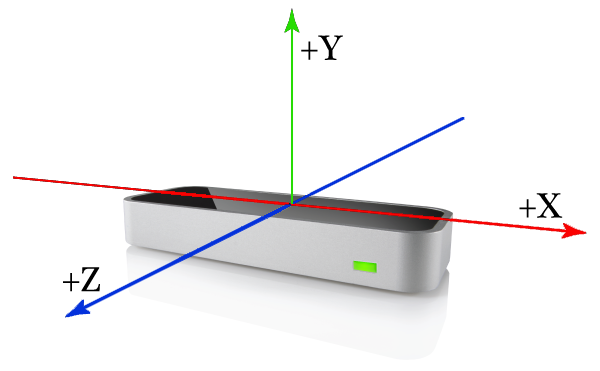
\includegraphics[width=6cm]{Leap-Axes}
                    \caption{The Leap Motion coordinate system. \cite{TAG11}}
                    \label{fig:leap1}
                \end{figure}
            
            \subsection{Unity Scripting API}
                Scripting is an essential ingredient in all video games. Even 
                the simplest game needs scripts, to respond to input from 
                the player and arrange for events in the gameplay to happen when 
                they should. 

                Our video game should be used a script to create graphical effects, 
                used to respond to input from player, control the physical behavior 
                of objects or even implement a custom AI system for characters 
                in the video game.
            
            \subsection{Unity importing object from blender}
                Creating beautiful and realistic object in Unity is too hard. 
                There are many programs make modeling easier and more realistic. 
                Blender is one of the most popular modeling 3D object program 
                because this program is easy to use and can import model to Unity.

                Unity natively imports Blender files, supporting 5 things. 
                First is all nodes with position, rotation and scale; pivot 
                points and names are also imported. Second is meshes with vertices, 
                polygons, triangles, UVs, and normals. Third is bones of character 
                or object. Fourth is skinned meshes. The last thing is animations. 
                They also have limitation such as Blender does not export the 
                visibility value inside animations in the FBX file. Our project 
                use limitation and functional of Blender to modeling good object 
                or character. We use Blender to make video game more interesting, 
                beautiful, and realistic.

            \subsection{Level Design Principle}
                Level design is a process of constructing the experiencethat will 
                be offered directly to the player, using components provided by 
                the game designer.

                Universal level design principle consist of 8 important rule that 
                guide game design that are:

                \begin{itemize}
                    \item   Game need to have tutorial level in order to make sure that 
                    player know how to play and explain the game interface, key 
                    challenges, and action
                
                    \item   Pacing of a level refers to the frequency at which the 
                    player encounters individual challenges. A fast pace can be 
                    create stress, offering challenge at a rapid rate

                    \item   Providing more resource, When the player surmounts a 
                    challenge that consumes his 	resources, provide more resource.
                    The player should not face another demanding challenge immediately 
                    after the player surmount a challenge that costs him a lot of resources
                    
                    \item   Avoid conceptual non-sequiturs creator should consider 
                    to build things that make sense. Don?t put dangers or reward 
                    in places in which no sane person could possibly expect to find them
                    
                    \item   Short-term goal creator should Clearly inform the player 
                    of his short-term goal and Should never leave your character 
                    wondering what to do next, the current or next short-term goal 
                    should be obvious
                    
                    \item   Be clear with risk, reward and then consequences of decisions. 
                    Player should not necessarily know every detail of what 
                    consequences his decisions will produce, the player should be 
                    able to make a reasonable guess based on the context.

                    \item   Skills, imagination, intelligence and dedication distinguish 
                    a good player. Good players deserve to be rewarded

                    \item   Primary objective is to give players an enjoyable experience. 
                    Build more rewards in to level than punishments

                    \item   The purpose of an artificial opponent is to put up a good 
                    fight and then lose Design level so that the player will get better 
                    and better at overcoming the challenges until he succeeds at all of them

                    \item Accessible to a wider audience by allowing them to switch the difficulty 
                    of your game to easy, normal or hard setting. And Be able to tweak the numbers 
                    to adjust the difficulty to accommodate the player?s preference

                \end{itemize}



            \subsection{Camera Image API}
                The Leap Motion controller uses infrared stereo cameras
                as tracking sensors. You can access the images from 
                these cameras using the \emph{Controller.images} or 
                \emph{Frame.images} functions. These functions provide 
                an \emph{ImageList} object, containing the Image objects. 
                \emph{Controller.images} provides the most recent set of images. 
                \emph{Frame.images} provides the set of images analysed to 
                create that frame and can be slightly older than the 
                images returned by the Controller directly. \\

                % Image and caption
                \begin{figure}[h]
                    \centering
                    
\includegraphics[width=4cm]{Leap-Image-Raw}
                    \caption{An image from one of the cameras. A grid highlighting 
                    the significant, complex distortion is superimposed on the image. \cite{TAG12}}
                    \label{fig:leapCam1}
                \end{figure}
                The images can be used for:
                \begin{itemize}
                    \item Head-mounted display video pass-through
                    \item Augmented reality
                    \item Computer vision 
                \end{itemize} 
                The Image API provides a buffer containing the sensor brightness
                values and a buffer containing the camera calibration map, 
                which can be used to correct lens distortion and other optical 
                imperfections in the image data.  \\

                \textbf{Image Distortion}

                When a ray of light enters one of the Leap Motion cameras, the 
                lens bends the light ray so that it hits the sensor, which records 
                it as a greyscale brightness value at a specific pixel location. 
                Of course, no lens is perfect, so a ray of light does not land 
                on the sensor in the optically perfect spot. The calibration 
                map provides data to correct this imperfection, allowing you to 
                calculate the true angle of the original ray of light. You can 
                use the corrected angle to generate a distortion-free image, and, 
                using the angles from both images in the stereo pair, you can 
                triangulate the 3D location of a feature identified in both images. 
                Note that the calibration map corrects lens distortion; it does 
                not correct perspective distortion.

                For image correction, the distortion data can be fed to a shader 
                program that can efficiently interpolate the correction applied to 
                rays of light. For getting the true angle for a small set of points, 
                you can use the \emph{Image.warp} function (but this is not efficient 
                enough to transform a full bitmap at a high frame rate).

                The distortion data is based on the angle of view of the Leap Motion 
                cameras. The image class provides functions, \emph{Image.RayScaleX} and 
                \emph{Image.RayScaleY} that are proportional to view angles large enough 
                to ensure that distortion map covers the entire view, about 150 degrees 
                for the current Leap Motion peripheral. A 150 degree angle of view means 
                that a light ray passing through the lens has a maximum slope of 4/1.

                \begin{figure}[h]
                    \centering
                    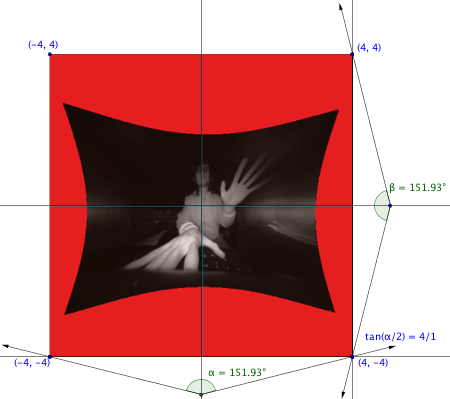
\includegraphics[width=5cm]{Leap-Image-Rays}
                    \caption{A view angle of 150 degrees corresponds to a slope of �4 
                    (The tangent of 75 degrees is approximately 4) \cite{TAG13}}
                    \label{fig:leapCam2}
                \end{figure}

        
        \begin{thebibliography}{1}

            \bibitem{TAG1}
                Elyoenai Guerra-Segura,Carlos M. Travieso and Jes�s B. Alonso, ?Study of the 
                variability of the Leap Motion?s measures for its use to characterize air strokes?, 
                \emph{in Measurement}, Vol. 105, pp. 87-97, July 2017
                
                
            \bibitem{TAG2}
                Catalin Constantin Moldovan and Ionel Staretu, ?An Anthropomorphic Hand with Five 
                Fingers Controlled by a Motion Leap Device?, \emph{in Procedia Engineering}, Vol. 181, 
                pp. 575-582, 2017
                

            \bibitem{TAG3}
                Christianne Falcao,Ana Catarina Lemos and Marcelo Soares, ?Evaluation of Natural User 
                Interface: A Usability Study Based on the Leap Motion Device?, 
                \emph{in Procedia Manufacturing}, Vol. 3, pp. 5490-5495, 2015
            
            \bibitem{TAG4}
                Dario Senkic, ?Dynamic Simulations in a 3D-Environment a comparison between Maya
                and Blender?, in Academy for technology and environment University of G�vle, 
                September 2010

            \bibitem{TAG5}
                Darran Jamieson, ?Making Difficult Fun: How to Challenge Your Players?, [Online]
                Available: https://gamedevelopment.
                tutsplus.com/tutorials/making-difficult-fun-how-to-challenge-your-players--cms-25873 [Accessed: May 20, 2016]
            
            \bibitem{TAG6}
                Michael B. and David H., ?Leap Motion API?, [Online] Available :
                https://developer.leapmotion.com/documentation/csharp/devguide/ \\
                Leap\textunderscore Overview.html 
                [Accessed: April 10, 2017]

            \bibitem{TAG7}
                Unity Technologies, ?Unity Scripting API?, [Online] Available :
                https://docs.unity3d.com/Manual/ScriptingSection.html [Accessed: April 5, 2018]
            
            \bibitem{TAG8}
                Unity Technologies, ?Importing Objects From Blender?, [Online] Available : 
                https://docs.unity3d.com/Manual/HOWTO-ImportObjectBlender.html [Accessed: April 5, 2018]

            \bibitem{TAG9}
                "General Principle of Level Design", [Online] Available :
                www.cas.mcmaster.ca/~se3gb3/SE3GB3/2014/slides/Chapter12.pptx
            
            \bibitem{TAG10}
                Michael B. and David H., ?Camera Image?, [Online] Available : 
                https://developer.leapmotion.com/documentation/csharp/devguide/ \\
                Leap\textunderscore Images.html 
                [Accessed: April 10, 2017]
             
             \bibitem{TAG11}
                Michael B. and David H., "Leap Axes", [Online] Available : 
                https://di4564baj7skl.cloudfront.net/documentation/images/Leap\textunderscore Axes.png
                [Accessed: April 10, 2017]
                
                \bibitem{TAG12}
                Michael B. and David H., "Leap Image Raw", [Online] Available : 
                https://di4564baj7skl.cloudfront.net/documentation/images/Leap\textunderscore Image\textunderscore Raw.png
                [Accessed: April 10, 2017]
                
                \bibitem{TAG13}
                Michael B. and David H., "Leap Image Rays", [Online] Available : 
                https://di4564baj7skl.cloudfront.net/documentation/images/Leap\textunderscore Image\textunderscore Rays.png 
                [Accessed: April 10, 2017]
	

        \end{thebibliography}


\end{document}
